%%%%%%%%%%%%%%%%%%%%%%%%%%%%%%%%%%%%%%%%%%%%%%%%%%%%%%%%%%%%%%%%%%%%%%%%%
% This file is part of the LaTeX sources of the OMDoc 1.2 specifiation
% Copyright (c) 2006 Louse Dennis, et al. 
% This work is licensed by the Creative Commons Share-Alike license
% see http://creativecommons.org/licenses/by-sa/2.5/ for details
\svnInfo $Id: main.tex 6161 2006-10-03 13:04:46Z  $
\svnKeyword $HeadURL: https://svn.omdoc.org/repos/omdoc/branches/omdoc-1.2/doc/spec/projects/induction-challenge/main.tex $
%%%%%%%%%%%%%%%%%%%%%%%%%%%%%%%%%%%%%%%%%%%%%%%%%%%%%%%%%%%%%%%%%%%%%%%%%

\section[Induction Challenge Problems]{Induction Challenge OMDoc Manager (ICOM)}

\begin{project}{induction-challenge}%
{http://www.cs.nott.ac.uk/~lad/research/challenges/challenge_manager.html}
\pauthors{Thomas D. Attfield\and 
  Monica C. Duarte\and 
  Lin Li\and 
  Ho-Ying Mak\and 
  Adam M. Neal\and 
  Lewis M. Toft\and 
  Zixuan Wang\and 
  Louise A. Dennis}
\pinstitute{School of Computer Science and Information Technology, University of Nottingham}
\end{project}

We describe work in progress to create a system for organising and presenting a set of
challenge problems\twin{induction}{challenge problems} collected by the Induction Theorem
Proving community.  These challenge problems come from a number of sources and are
presented in different logics using different presentation conventions.

The intention is to provide a system which will allow these problems
to be stored in a unified format and will support the collection,
browsing and extraction of the problems.

{\omdoc} is an obvious choice for representing such problems and the system is able to
take advantage of much existing work on the manipulation of {\xml} documents.

\subsection{The Induction Challenge Problems}
Inductive Theorem proving\twin{induction}{theorem prover} is a small field.  The main
theorem provers within this field are {\nqthm}~\cite{NQTHM} (now re-engineered as
{\acltwo}~\cite{kaufmann96acl}), {\inka}~\cite{INKA5}, the {\clam}
series~\cite{pub507,lclamsysdesc} and {\scsys{rrl}}~\cite{kapur95overview}.
{\twelf}~\cite{pfenning99system} also looks at the automation of inductive proof in the
context of \twintoo{logical}{framework}s.  Within the field it is hard to assess claims
for the superiority of any given system since there is naturally a tendency to report
``successes'' -- difficult or challenging problems automatically proved.  There is also a
desire within the community to develop a store of shared knowledge about the challenges
that face the automation of proof by mathematical induction.

{\indextoo{TPTP}} (Thousands of Problems for Theorem Provers\index{theorem
  prover}s)~\cite{Sutcliffe98} is a library of test problems for first-order
{\indextoo{ATP}} systems\atwin{first-order}{theorem}{prover}. They provide the ATP
community with a comprehensive library complete with unambiguous names and references.
All the problems are stated in a standardised formulation of
{\twintoo{first-order}{logic}} and are widely used to benchmark first-order systems.  They
are also used as the test set for the {\indextoo{CASC competition}}~\cite{Sutcliffe01} which
compares such systems.  One of the benefits of the TPTP library to the ATP community is
the existence of a common set of problems by which comparisons can be made.

It is not practical for inductive theorem provers\twin{induction}{theorem provers} to
follow the pattern of the {\indextoo{TPTP}} library.  Various attempts have been made to
build a similar corpus of problems requiring inductive reasoning.  The most mature of
these was based on the Boyer-Moore~\cite{NQTHM}
corpus\twin{Boyer-Moore}{corpus}\footnote{This has become known as the
  {\twintoo{Dmac}{corpus}} after David McAllester who translated a fragment of the
  {\nqthm} corpus into a simpler language.}.  This corpus was unpopular partly because
there was repetition within the problem set and partly because many problems depended on a
few particular function definitions.  But the major objection was that
{\twintoo{induction}{theorem prover}s} use a number of different logics, some of which are
typed and some of which are not, which made it difficult to agree on a standard format.
The use of other logics also raised translation issues and a fully automated process for
converting the theorems, even into an agreed typed language was never produced.

A group of researchers within the community\footnote{At the 2000 CADE Workshop on the
  Automation of Proof by Mathematical Induction.}  agreed that instead of a large set of
benchmarks in a standard logic they would each put forward a number of ``Challenge
Problems''\twin{induction}{challenge problems}.  These should present interesting
challenges to the automation of inductive proof or illustrate important features which an
inductive prover should be able to handle.  A set of these problems would be collected
which would remain sufficiently small that an individual could represent them within their
own theorem proving system as they saw fit\footnote{The current set can be found at
  {\url{http://www.cs.nott.ac.uk/~lad/research/challenges}}.}.  These challenge problems
are currently described in a high-level way and written up in an ad hoc fashion.  The
descriptions contain both mathematical notation and commentary.  They are difficult to
read, navigate or use in any particular system.

{\omdoc} seems ideally suited as a format for representing these challenge
problems\twin{induction}{challenge problems}: it can represent both text and formulae; it
is not tied to any particular logic and it supports the extraction of data into a number
of different formats.  As an added benefit its hyper-text features would potentially allow
definitions to be stored separately and shared between problems.  Individual theorem
provers\twin{induction}{theorem provers} can then concentrate on translations between
{\openmath} content dictionaries\atwin{OpenMath}{content dictionaries} and their own
logics and individuals submitting problems can specify the appropriate content dictionary
for the problem.

\subsection{System Description}
The Induction Challenge {\omdoc} Manager (\scsys{ICOM}) is designed to be a system which
will ease the submission and extraction process for the problems.  Our intention is to
provide a submission interface that will create a simple {\omdoc} markup for the problems
which can subsequently be edited by a user and to provide browsing and extraction
capabilities.

Each challenge problem description contains six distinct sections (e.g. Summary,
Definitions, Comments).  Currently a user who wishes to enter a problem into our system is
presented with the form shown on the right with a field for each section.  

\begin{wrapfigure}{r}{2in}
  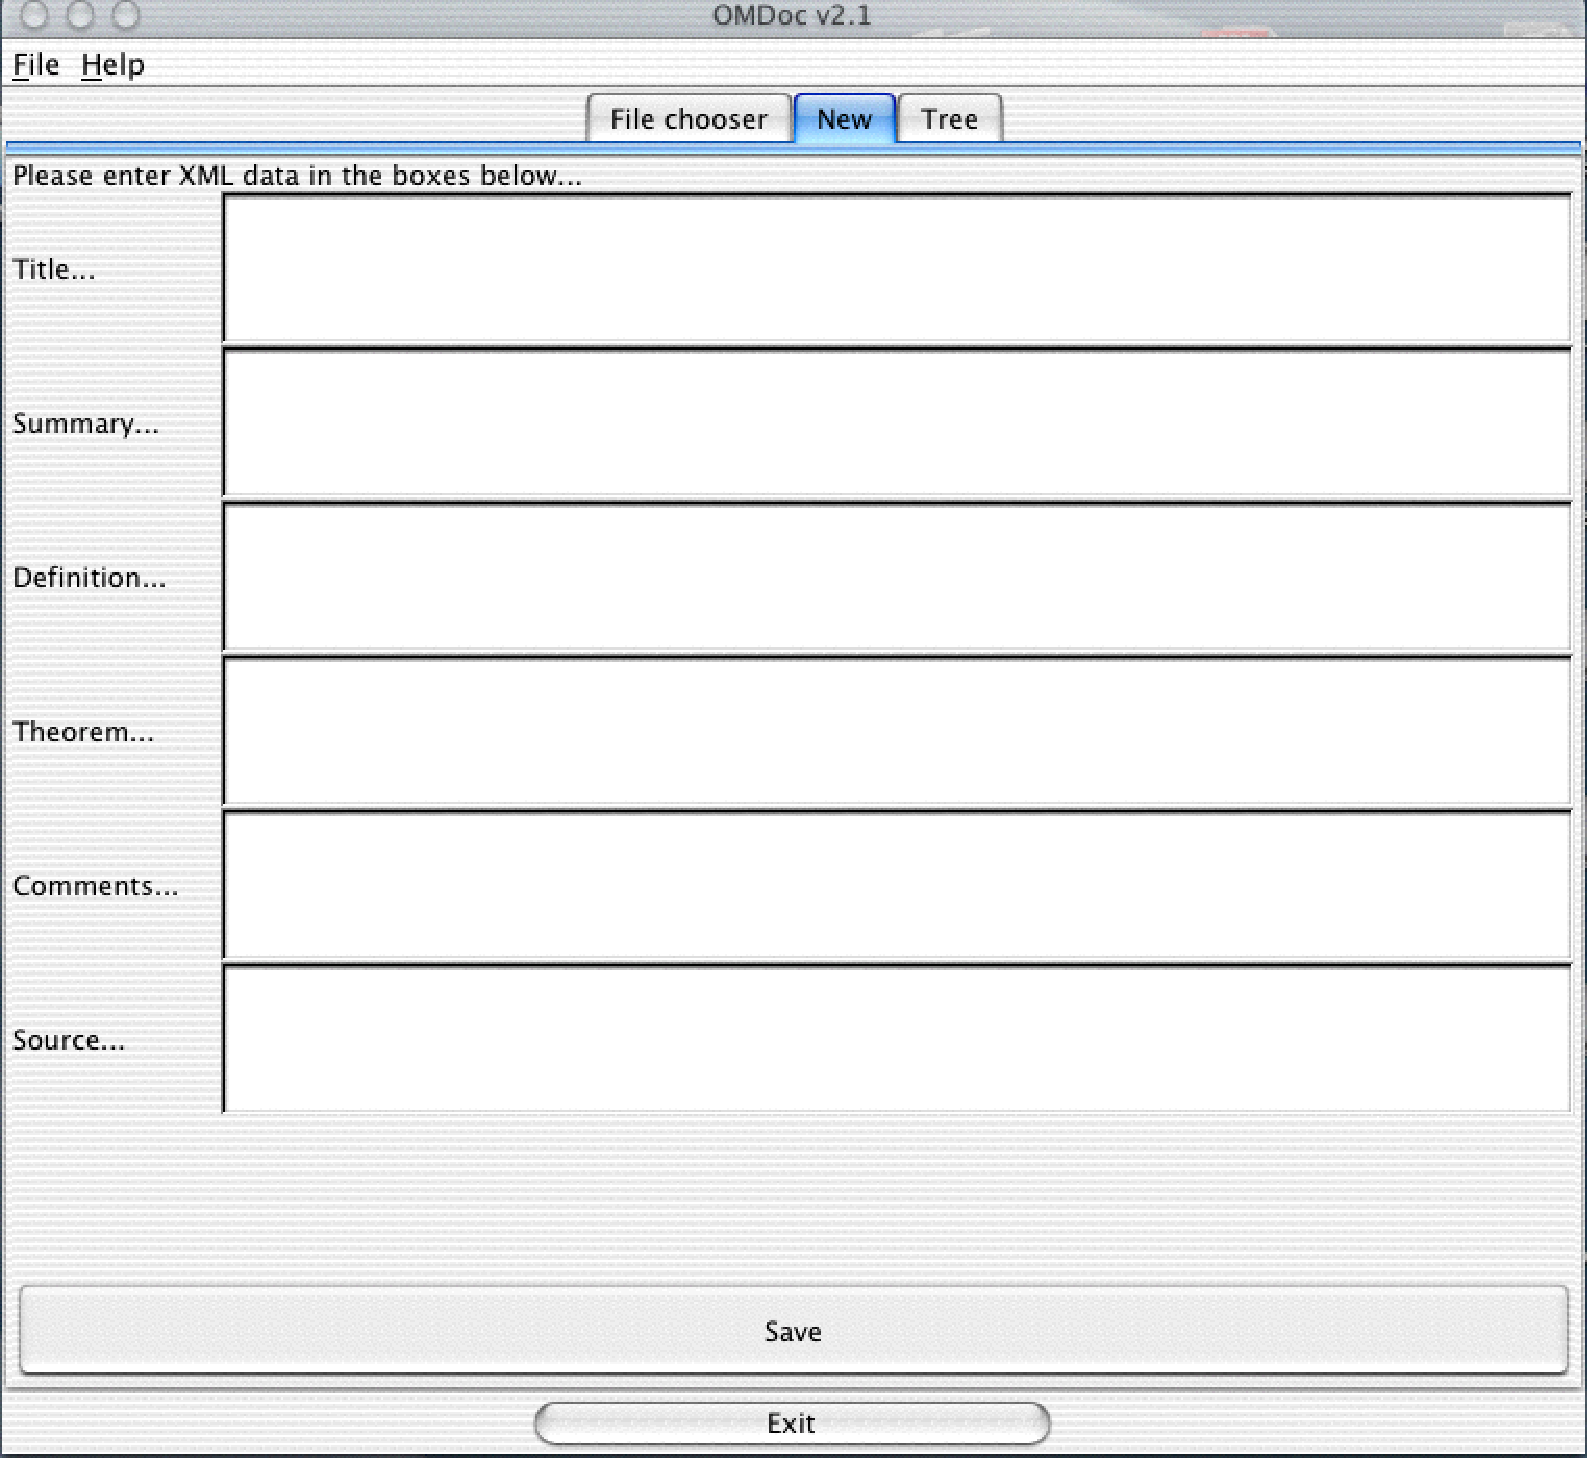
\includegraphics[width=2in]{projects/induction-challenge/inputview}
\end{wrapfigure}
Each section, once entered by a user, is placed in a {\element{CMP}} tag.  These tagged
fragments are wrapped in standard {\omdoc} headers and footers to produce a valid
{\omdoc}. This completed document is then written to disk and stored.  We are currently
working on a simple parser to translate equations into \element[ns-elt=om]{OMOBJ} structures which a
user will then be able to edit (for instance to specify the appropriate content
dictionaries).  We hope this will be easier than adding all the {\openmath} tags by hand.

An existing document can be displayed as a tree and from this tree the document can be
directly manipulated. This tree display also allows the user to see the structure of the
document more clearly.  It is also possible to extract an HTML view of the contents of the
document so it can be displayed in a web browser and read by a human.

\begin{wrapfigure}{r}{2in}
  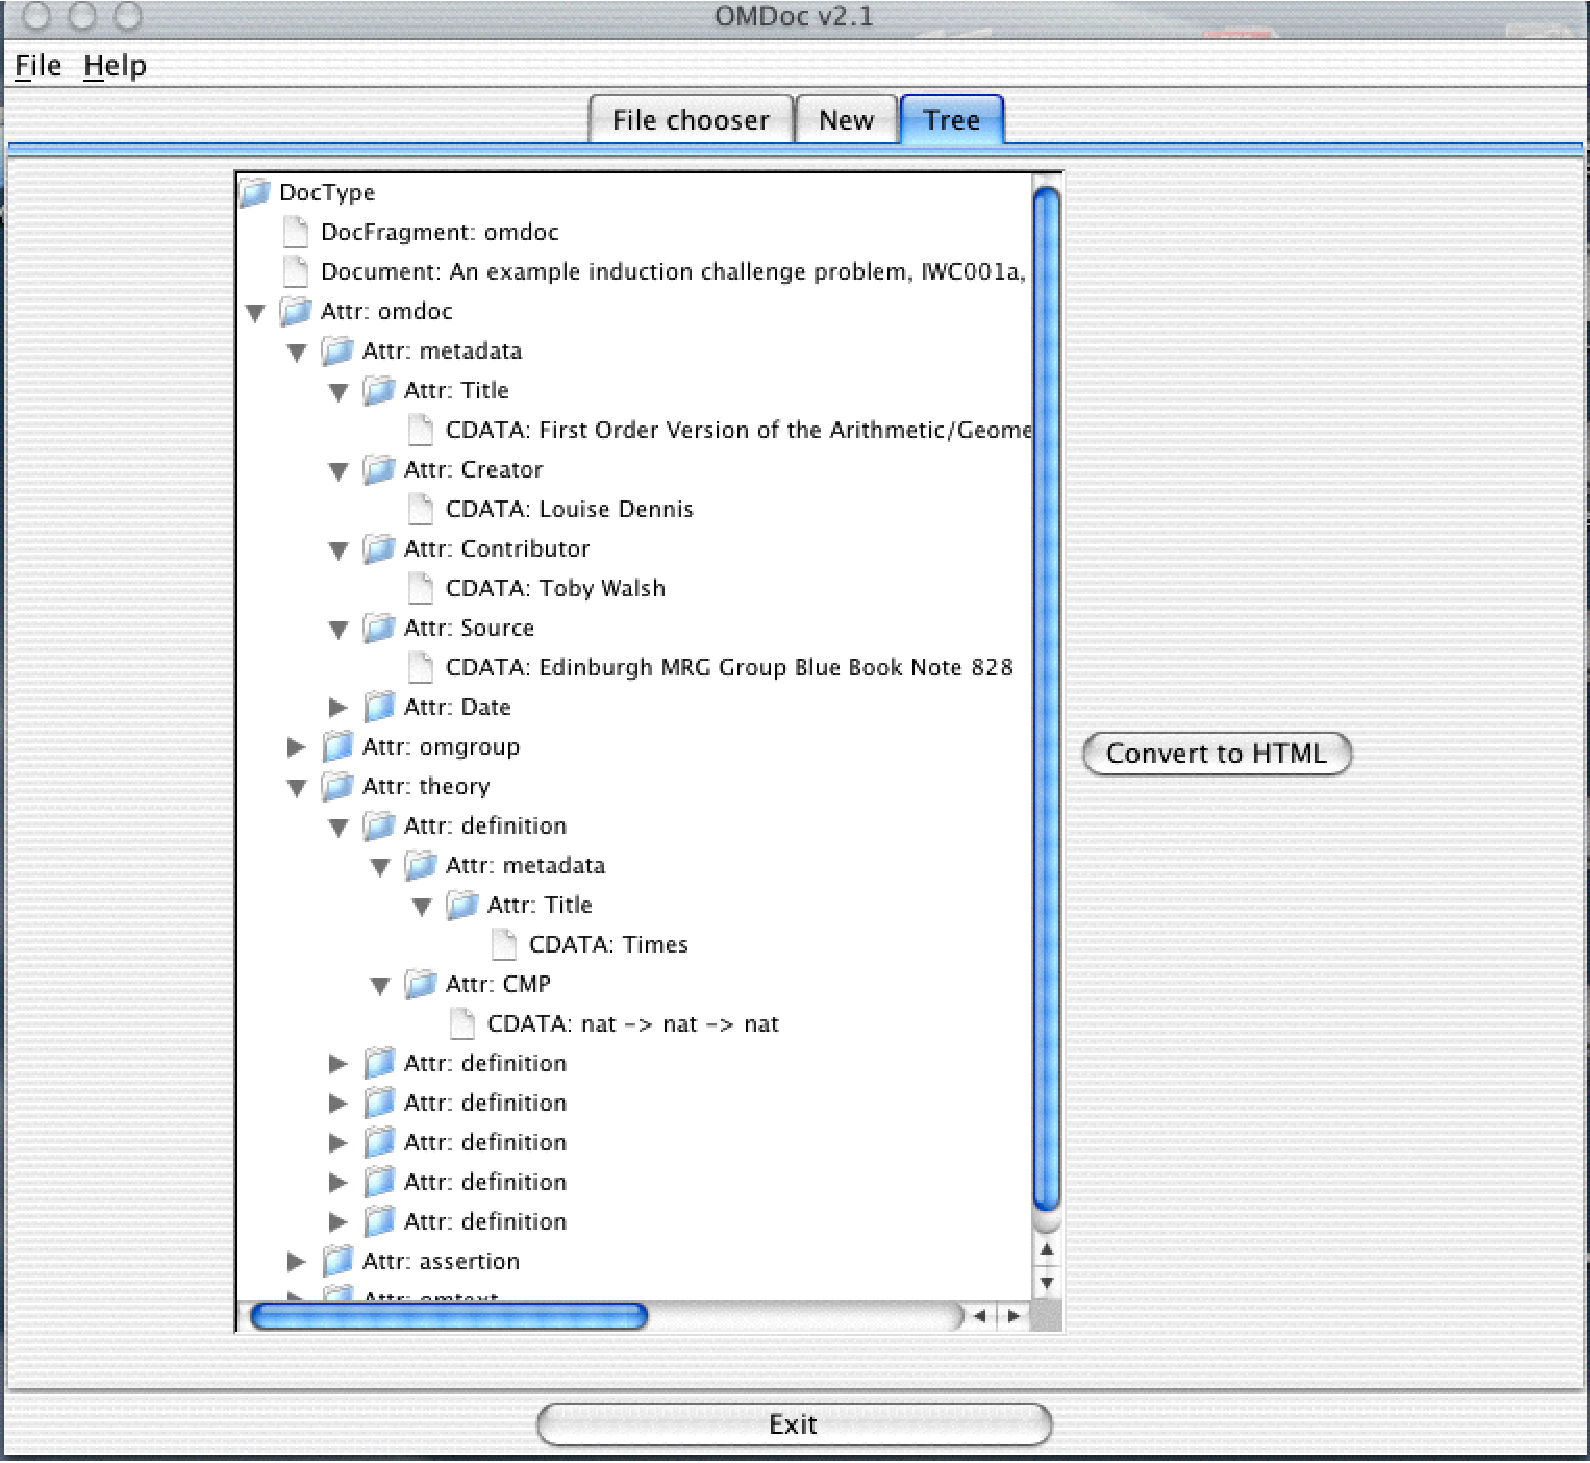
\includegraphics[width=2in]{projects/induction-challenge/treeview}
\end{wrapfigure}
Our implementation language is {\java} and we use its {\twintoo{JAXP}{DOM}} API.
{\indextoo{DOM}}~\cite{URL:DOM} is a W3C standard which uses a tree-based model (storing
data in hierarchies of nodes).  This means that once an {\omdoc} has been created or
opened all the document's data is in memory and so data can be accessed rapidly. DOM also
enables simple modification of documents by adding or deleting nodes.  Although {\sax} (an
alternative model) achieves better performance and less memory overhead than DOM, it is
easier to traverse and modify XML documents using a DOM tree structure.  Since we
anticipate that users may wish to modify the initial {\omdoc} produced by our system we
adopted the DOM model instead.

\subsection{Further Work} {\scsys{ICOM}} is still in the early stages of development.
Currently our most pressing aim is to provide improved support for entering equations.
Once this is in place we hope to add searching facilities and provide better mechanisms
for links to be created between challenge problems.  We would also like to experiment with
the automatic extraction of problems into a theorem prover via an
{\mbase}~\cite{KohlhaseFranke00} and a {\mathweb}~\cite{MathWeb99}.

%%% Local Variables: 
%%% mode: latex
%%% TeX-master: "../../omdoc"
%%% End: 

% LocalWords:  ICOM Attfield Duarte Ying Mak Toft Zixuan rrl TPTP CASC Dmac hoc
% LocalWords:  McAllester CADE ns elt JAXP API
